\documentclass{beamer}

\usepackage{framed}
\usepackage{graphicx}

\begin{document}
\section{Plotting a regression in other contexts}
%===========================================================%
\begin{frame}[fragile]
\frametitle{Seaborn Workshop}
\large
\noindent \textbf{Plotting a regression in other contexts}
	\begin{itemize}
\item A few other seaborn functions use \texttt{regplot()} in the context of a larger, more complex plot. 
\item The first is the \texttt{jointplot()} function that we introduced in the distributions tutorial.
\item In addition to the plot styles previously discussed, \texttt{jointplot()} can use \texttt{regplot()} to show the linear regression fit on the joint axes by passing \texttt{kind="reg"}:
\end{itemize}
\end{frame}
%===========================================================%
\begin{frame}[fragile]
\frametitle{Seaborn Workshop}
	\large

\begin{verbatim}
sns.jointplot(x="total_bill", y="tip", 
              data=tips, kind="reg");
\end{verbatim}

\begin{figure}
\centering
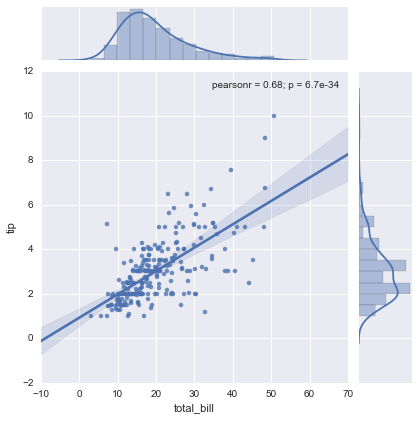
\includegraphics[width=0.60\linewidth]{images/regression_51_0}
\end{figure}
\end{frame}
%===========================================================%
\begin{frame}[fragile]
	\frametitle{Seaborn Workshop}
	\large
\begin{itemize}
\item Using the \texttt{pairplot()} function with \texttt{kind="reg"} combines \texttt{regplot()} and \texttt{PairGrid} to show the linear relationship between variables in a dataset.
\item Take care to note how this is different from \texttt{lmplot()}. 
\item In the figure below, the two axes don’t show the same relationship conditioned on two levels of a third variable; rather, \item \texttt{PairGrid()} is used to show multiple relationships between different pairings of the variables in a dataset:
\end{itemize}

\end{frame}
%===========================================================%
\begin{frame}[fragile]
	\large
\begin{verbatim}
sns.pairplot(tips, x_vars=["total_bill", "size"],  
       y_vars=["tip"], size=5, aspect=.8, kind="reg");
\end{verbatim}
\begin{figure}
\centering
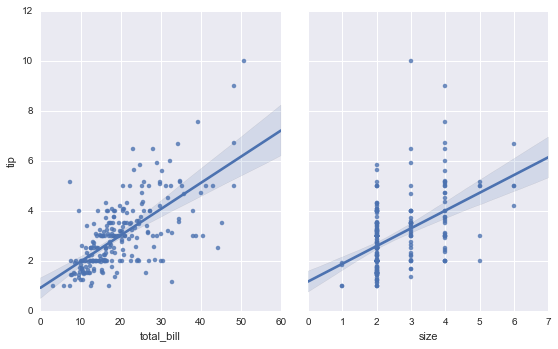
\includegraphics[width=0.8\linewidth]{images/regression_53_0}
\end{figure}

\end{frame}
%===========================================================%
\begin{frame}[fragile]
	\frametitle{Seaborn Workshop}
	Like lmplot(), but unlike jointplot(), conditioning on an additional categorical variable is built into pairplot() using the hue parameter:
\begin{verbatim}
sns.pairplot(tips, x_vars=["total_bill", "size"], y_vars=["tip"],
             hue="smoker", size=5, aspect=.8, kind="reg");

\end{verbatim}
\begin{figure}
	\centering
	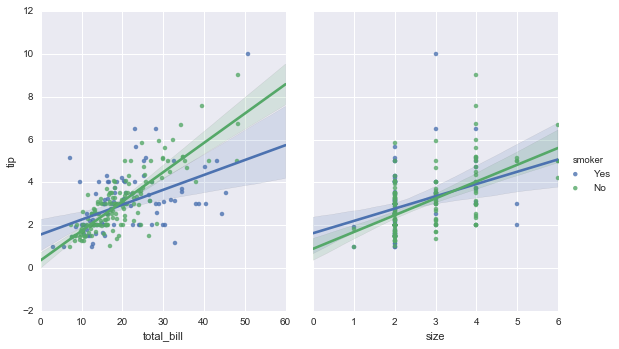
\includegraphics[width=0.8\linewidth]{images/regression_55_0}
\end{figure}
\end{frame}

\end{document}